% !TeX root = ../tfg.tex
% !TeX encoding = utf8

\chapter{Evolución del Deep Double Descent}\label{sec:evolucion-ddd}

El \emph{Deep Double Descent}, al ser un fenómeno estrechamente relacionado al avance tecnológico y al crecimiento en la capacidad y el tamaño de los modelos de aprendizaje profundo, ha despertado un mayor interés en los últimos años, como puede observarse en la~\autoref{fig:histogram}. No obstante, aunque se percibe, durante los últimos años, una tendencia al alza del número de publicaciones que hacen referencia al citado fenómeno, únicamente encontramos un total 143 publicaciones en Scopus\footnote{Encontradas 143 publicaciones a fecha 10 de febrero de 2025 usando la consulta: TITLE-ABS-KEY (deep AND double AND descent).}. Esta reciente relevancia del fenómeno ilustra el carácter \textbf{innovador} y \textbf{pionero} de este proyecto.\newline

\begin{figure}[h]
    \centering
    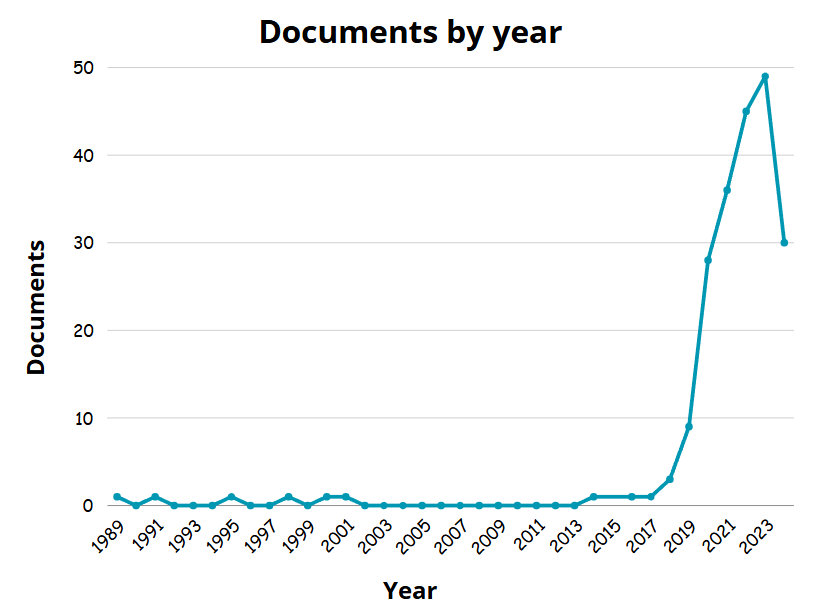
\includegraphics[width=0.8\linewidth]{img/scopus_histogram.png}
    \caption[Número de publicaciones relativas al Deep Double Descent (ir actualizando histograma de cara a nuevos papers).] {Número de publicaciones relativas al Deep Double Descent en función del año de publicación.}\label{fig:histogram}
\end{figure}

Sin embargo, aunque la cantidad de artículos científicos sobre este fenómeno aún sea limitada, el interés por parte de investigadores y científicos está creciendo rápidamente. Incluso en ausencia de publicaciones científicas formales, se continúan obteniendo nuevos resultados, tanto teóricos como prácticos, que continúan enriqueciendo nuestra comprensión del problema. De hecho, en Scopus\footnote{Encontradas 105 preimpresiones a fecha 10 de febrero de 2025 usando la consulta: TITLE-ABS-KEY (deep AND double AND descent).}, podemos encontrar 105 preimpresiones relacionadas con el fenómeno.\newline

A pesar de la disponibilidad de artículos que abordan este fenómeno, la mayoría de ellos no proporcionan una explicación detallada del mismo, centrándose generalmente en casos prácticos y dejando de lado el análisis teórico subyacente, que se encuentra detrás de los resultados obtenidos, lo que limita la comprensión completa de ciertos aspectos del fenómeno.\newline

\section{Origen y primeras manifestaciones del fenómeno}\label{}

Aunque la primera publicación formal sobre el \emph{Deep Double Descent} data de 1996, como se observa en la~\autoref{fig:histogram}, el fenómeno parece haber sido descrito por primera vez en la literatura de la física teórica en 1989, aunque de manera superficial y sin la denominación actual. Por ello, nos remontamos hasta 1995 cuando Opper presenta este resultado en su artículo ``Statistical Mechanics of Generalization''~\cite{Opper1995}, a través del uso de una red neuronal formada por un perceptrón de una sola capa con una función de activación lineal conocida como ADALINE~\cite{WidrowHoff1960}, y, más tarde, en su revisión del artículo en 2001 ``Learning to Generalize''~\cite{Opper2001}.\newline

\begin{figure}[h]
    \centering
    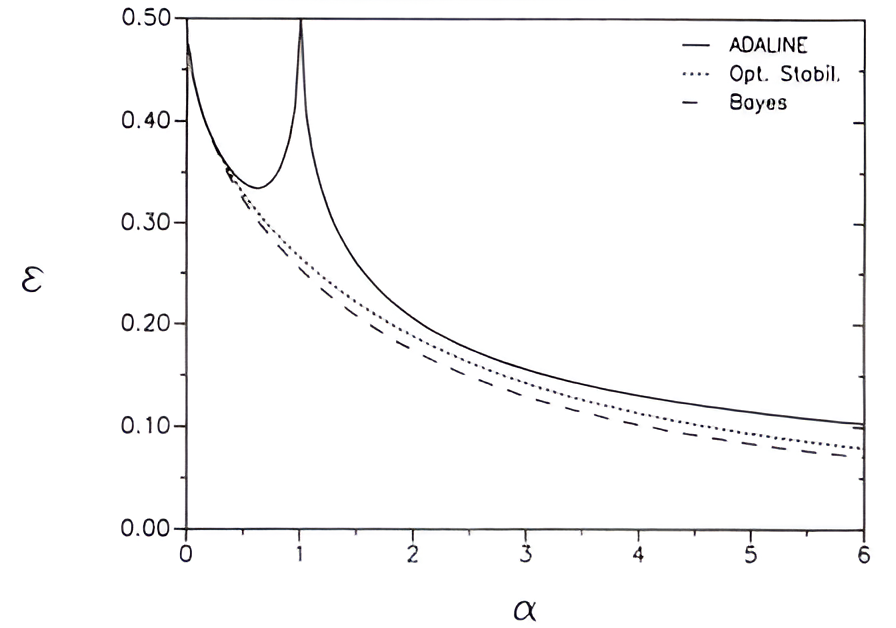
\includegraphics[width=0.8\linewidth]{img/estadoarte2.png}
    \caption[Deep Double Descent presente en ADALINE.]{Comparación del error de generalización ($\epsilon$) para distintos modelos en función de la fracción entre el número de ejemplos aprendido y el número de parámetros ($\alpha$). Se observa la curva del doble descenso para el modelo ADALINE~\cite{Opper1995}.}\label{fig:estadoarte2}
\end{figure}

En ambos artículos, Opper presenta de manera gráfica el fenómeno del doble descenso utilizando un modelo neuronal lineal (denominado así por el uso de funciones de activación lineales), aunque sin profundizar demasiado en este resultado (véase~\autoref{fig:estadoarte2}). En sus representaciones, el error de generalización ($\epsilon$) se muestra en función del número de ejemplos de entrenamiento ($n$) y el número de parámetros ($P$), donde $\alpha = \frac{n}{P}$. Se observa que el error de generalización alcanza su pico cuando $\alpha$ se aproxima a 1, es decir, cuando el número de ejemplos de entrenamiento es similar al número de parámetros del modelo.\newline

Comportamientos similares a los obtenidos por Opper también han sido reportados por Advani \& Saxe en~\cite{Advani2017}, Spigler et al. en~\cite{Spigler2019} y Geiger et al. en~\cite{Geiger2019}. Estos trabajos, anteriores a la formalización del fenómeno tal como se conoce hoy en día, trabajan con redes neuronales profundas con un gran número de parámetros y estudian el comportamiento del error de generalización utilizando herramientas de física estadística inspiradas en el trabajo de Opper. Además,~\cite{Spigler2019} y~\cite{Geiger2019} proponen una conexión entre el fenómeno y la transición de jamming propia de la física estadística, mostrando por qué los modelos pueden llegar a generalizar mejor después del pico del error de prueba. Sin embargo, fue Duin (2000) en~\cite{Duin2000} (véanse Figuras 6 y 7) el primero en mostrar curvas de generalización, utilizando datos del mundo real, bastante similares a las curvas del doble descenso que tenemos hoy en día.\newline

\section{El nacimiento del Deep Double Descent}\label{}

Iniciamos esta sección abordando el equilibrio clásico entre sesgo y varianza, un concepto fundamental en la teoría del aprendizaje automático (\cite{Geman1992},~\cite{Hastie2001} y~\cite{Bengio2010}). Esta teoría sostiene que, a medida que la complejidad de un modelo aumenta, su sesgo disminuye, pero su varianza se incrementa. Como resultado, llega un punto en el que el modelo comienza a sobreajustar, lo que provoca un aumento en el error de generalización, dominado por la varianza y la tradicional curva en forma de ``U'' del error de generalización. De acuerdo con esta visión tradicional, una vez superado cierto umbral de complejidad, los modelos más grandes son cada vez peores y, por tanto, se busca encontrar un equilibrio en el modelo.\newline

Sin embargo, los resultados prácticos modernos no comparten esta teoría. En la actualidad, la visión moderna entre los profesionales es que los \emph{modelos grandes son mejores} (\cite{Krizhevsky2012},~\cite{Neal2019},~\cite{Huang2019},~\cite{Szegedy2014}). Estos estudios muestran que el uso de redes neuronales con un gran número de parámetros conduce a un mejor rendimiento, evidenciando que los modelos más complejos pueden obtener resultados superiores a los modelos simples. Por ello, este trabajo se enmarca dentro del estudio de la generalización en redes neuronales profundas. En particular, se enlaza con investigaciones previas, como la de Zhang et al. (2021) en~\cite{Zhang2021}, quienes argumentan que comprender el aprendizaje profundo aún requiere replantearse los paradigmas tradicionales de generalización, desafiando la noción clásica de sesgo-varianza.\newline

El fenómeno del \emph{Deep Double Descent} fue nombrado así, por primera vez, por Belkin et al.\ en~\cite{Belkin2019}, haciendo referencia a los dos descensos que presenta la curva del error de generalización. En este artículo, se busca unificar la teoría clásica del equilibrio sesgo-varianza con los resultados prácticos obtenidos por la teoría moderna, mediante una curva de error unificada (véase~\autoref{fig:estadoarte2.2}).\newline

\begin{figure}[h]
    \centering
    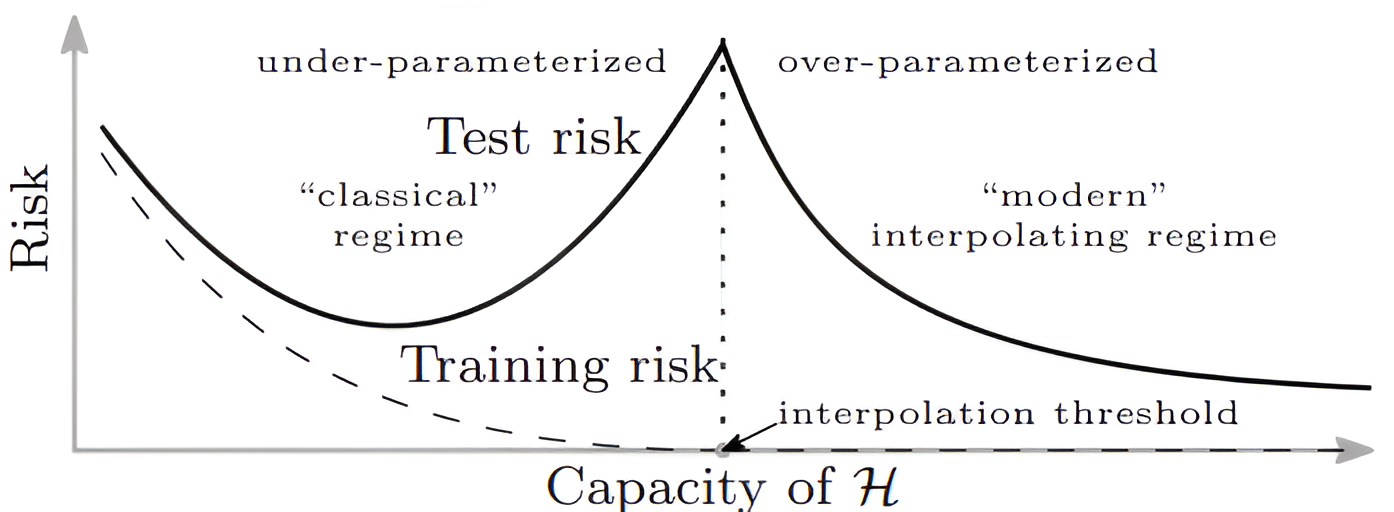
\includegraphics[width=0.8\linewidth]{img/estadoarte2.2.png}
    \caption[Curva del error unificada entre la teoría clásica y moderna.]{Curvas para el error de entrenamiento (línea discontinua) y el error de generalización (línea continua). Antes del umbral de interpolación, se muestra la curva clásica en ``U''. Después de dicho umbral, se observa la curva del error moderna, induciendo el doble descenso. Imagen obtenida de~\cite{Belkin2019}.}\label{fig:estadoarte2.2}
\end{figure}

Belkin et al.\ muestra la aparición del fenómeno en diversos conjuntos de datos y con distintos tipos de modelos, entre los que se incluyen los árboles de decisión y redes neuronales con dos capas ocultas. Además, ofrece una primera intuición sobre su causa, argumentando que, en la región sobreparametrizada, el modelo dispone de un mayor número de funciones candidatas compatibles con los datos. A esto se suma el efecto de la regularización implícita inducida por ciertos algoritmos de optimización, como el gradiente descendente (\cite{Soudry2024}).\newline

Posteriormente, Nakkiran et al.\ (\cite{Nakkiran2019}) observaron que el fenómeno del doble descenso no solo dependía del tamaño del modelo, sino también del número de épocas de entrenamiento. Además, unificaron estos resultados mediante la introducción de una nueva medida de complejidad para un modelo: la \textbf{complejidad efectiva del modelo}, y conjeturaron bajo qué condiciones este fenómeno podía ocurrir en función de dicha medida. En este mismo trabajo, también formalizaron los distintos tipos de doble descenso que pueden manifestarse: en función del número de parámetros, del número de épocas y del tamaño del conjunto de entrenamiento y que será la base conceptual sobre la que desarrollaremos este proyecto.\newline

\section{Avances recientes del Deep Double Descent}\label{}

En los últimos años, la comprensión del fenómeno del \textit{Deep Double Descent} ha avanzado significativamente, con nuevas investigaciones que han refinado su caracterización y explorado sus implicaciones en redes neuronales profundas.\newline

Uno de los principales avances en el campo del aprendizaje estadístico ha sido la reconsideración de los límites de la sabiduría clásica sobre el sesgo y la varianza, especialmente al analizar el impacto del uso de un gran número de parámetros en el aprendizaje (\cite{Zhang2021},~\cite{Curth2023}). Por otro lado, Schaeffer et al. (2023) (\cite{Schaeffer2023}) realizaron los primeros estudios teóricos y experimentales enfocados en identificar y analizar las posibles causas y factores que pueden desencadenar el fenómeno.\newline

Otras líneas de investigación han explorado cómo ciertas técnicas pueden mitigar el doble descenso. Por ejemplo, Yang y Suzuki (2023) en~\cite{Yang2024} analizaron el impacto de la regularización mediante el uso de dropout, demostrando que dicha técnica puede reducir la magnitud del segundo descenso en el error de generalización. Asimismo, Heckel y Yilmaz (2021) en~\cite{Heckel2020} investigaron cómo el uso de la parada anticipada \emph{o early stopping} puede influir en el fenómeno.\newline

Desde una perspectiva más empírica, varios estudios han analizado la manifestación del fenómeno en escenarios de aprendizaje adversario. En particular, Min et al. (2021) en~\cite{Ming2020} demostraron que, en algunos casos, un aumento de los datos de entrenamiento puede mejorar la robustez del modelo, aunque también puede provocar un descenso adverso en la generalización. Asimismo, Singh et al. (2022) en~\cite{Singh2022} presentaron un análisis teórico del fenómeno en redes neuronales de tamaño finito (con un número finito de neuronas por capa y que no son capaces de memorizar el conjunto de entrenamiento), proporcionando una caracterización matemática básica que ayuda a entender los mecanismos subyacentes. Por último, Somepalli et al. (2022) en~\cite{Somepalli2022} investiga la reproducibilidad del aprendizaje en redes neuronales y su relación con el doble descenso.\newline

Finalmente, investigaciones recientes han mostrado extensiones del fenómeno, pues el fenómeno del doble descenso no está necesariamente limitado a dos descensos, sino que, bajo ciertas circunstancias, pueden observarse más de dos descensos (~\cite{d_Ascoli2021}, ~\cite{Chen2021}). Además, se ha estudiado la relación del doble descenso con otros fenómenos emergentes en el aprendizaje profundo, como es el caso del \emph{grokking}. En este contexto, Davies et al. (2023) en~\cite{Davies2023} propusieron una conexión entre ambos, sugiriendo que el aprendizaje prolongado puede llevar a una mejora abrupta de la generalización, similar a lo que ocurre en zona sobreparametrizada del fenómeno.\newline

\endinput